\documentclass[10pt,leter,openany]{article}
\usepackage[latin1]{inputenc}
\usepackage[english]{babel}
\usepackage{amsmath}
\usepackage{amsfonts}
\usepackage{amssymb}
\usepackage{graphicx}
\usepackage{listings}
\usepackage{color}
\usepackage[left=3cm,right=3cm,top=3cm,bottom=3cm]{geometry}
\usepackage[numbers,sort&compress]{natbib}
\usepackage{url}
\usepackage{caption}
\usepackage{siunitx}
%\usepackage{subfigure}
\usepackage{float}
\usepackage{booktabs}
\usepackage{subcaption}
\usepackage{comment}
\usepackage{mwe}
%\usepackage[table,xcdraw]{xcolor}

\setlength{\parindent}{0pt}
\setlength{\parskip}{4pt}

\definecolor{mygreen}{rgb}{0,0.6,0}
\definecolor{mygray}{rgb}{0.5,0.5,0.5}
\definecolor{mymauve}{rgb}{0.58,0,0.82}

\lstset{ 
	backgroundcolor=\color{white},   % choose the background color; you must add \usepackage{color} or \usepackage{xcolor}; should come as last argument
	basicstyle=\footnotesize,        % the size of the fonts that are used for the code
	breakatwhitespace=false,         % sets if automatic breaks should only happen at whitespace
	breaklines=true,                 % sets automatic line breaking
	captionpos=b,                    % sets the caption-position to bottom
	commentstyle=\color{mygreen},    % comment style
	deletekeywords={...},            % if you want to delete keywords from the given language
	escapeinside={\%*}{*)},          % if you want to add LaTeX within your code
	extendedchars=true,              % lets you use non-ASCII characters; for 8-bits encodings only, does not work with UTF-8
	firstnumber=01,                	 % start line enumeration with line 1000
	frame=single,	                 % adds a frame around the code
	keepspaces=true,                 % keeps spaces in text, useful for keeping indentation of code (possibly needs columns=flexible)
	keywordstyle=\color{blue},       % keyword style
	language=Python,                 % the language of the code
	morekeywords={*,...},            % if you want to add more keywords to the set
	numbers=left,                    % where to put the line-numbers; possible values are (none, left, right)
	numbersep=5pt,                   % how far the line-numbers are from the code
	numberstyle=\tiny\color{mygray}, % the style that is used for the line-numbers
	rulecolor=\color{black},         % if not set, the frame-color may be changed on line-breaks within not-black text (e.g. comments (green here))
	showspaces=false,                % show spaces everywhere adding particular underscores; it overrides 'showstringspaces'
	showstringspaces=false,          % underline spaces within strings only
	showtabs=false,                  % show tabs within strings adding particular underscores
	stepnumber=1,                    % the step between two line-numbers. If it's 1, each line will be numbered
	stringstyle=\color{mymauve},     % string literal style
	tabsize=2,	                     % sets default tabsize to 2 spaces
	title=\lstname                   % show the filename of files included with \lstinputlisting; also try caption instead of title
}

\usepackage[dvipsnames,table,xcdraw]{xcolor}

\usepackage{fancyvrb}

% redefine \VerbatimInput
\RecustomVerbatimCommand{\VerbatimInput}{VerbatimInput}%
{fontsize=\footnotesize,
	%
	frame=lines,  % top and bottom rule only
	framesep=2em, % separation between frame and text
	rulecolor=\color{Gray},
	%
	label=\fbox{\color{Black}data.txt},
	labelposition=topline,
	%
	commandchars=\|\(\), % escape character and argument delimiters for
	% commands within the verbatim
	%commentchar=*        % comment character
}



\usepackage{titling}
\newcommand{\subtitle}[1]{%
	\posttitle{%
		\par\end{center}
	\begin{center}\large#1\end{center}
	\vskip0.5em}%
}


\author{5273}
\title{Homework Assignment 8: Applied Probabilistic Models}
\subtitle{Bayes' Theorem}
\date{}


\begin{document}
	
\maketitle

\section{Introduction}

		In this work, are analyzed some applications of Bayes' theorem. Several documents discuss the interpretation of Bayes' theorem in  COVID-19 test results and its true accuracy and how data can be interpreted in subjects which have been tested to find out if have the disease. Several of these documents prove how applying Bayes' theorem may lead to counterintuitive results.
	
	
	For the analysis, the R software is used in its version 4.0.2 \citep{r}, and the code used is available on the GitHub repository of  \citep{github}. This work is run on a MacBook Air with an Intel Core i5 CPU $ @ $ 1.8 GHz and 8 GB RAM.
	
	
\section{Document discussion}

	To begin with, some basic concepts treated in the documents need to be reviewed, adapted with COVID-19  tests.
	
	\begin{enumerate}
		\item True positive: A person with COVID-19 tests positive for COVID-19.
		\item False positive: A person without COVID-19 tests positive for COVID-19.
		\item False negative: A person with COVID-19 tests negative for COVID-19.
		\item True negative: A person without COVID-19 tests negative for COVID-19.
	\end{enumerate}

	The term sensitivity is the probability that a person tests positive, given that they have the disease. The specificity is the probability that a person tests negative, given that they do not have the disease; also, the terms accuracy and precision can be resumed in Table \ref{tab:concepts}.

\begin{table}[]
	\centering
	\caption{Concepts about tests}
	\label{tab:concepts}
	\begin{tabular}{@{}ll@{}}
		\toprule
		\textbf{Concept}     & \textbf{Interpretation}                                                         \\ \midrule
		Accuracy    & $ \frac{\mbox{true positives + true negatives}}{\mbox{all results}}$  \vspace{0.5cm} \\
		Precision   & $ \frac{\mbox{true positives}}{\mbox{true positive + false positive}}$ \vspace{0.5cm} \\
		Sensitivity & $ \frac{\mbox{true positives}}{\mbox{true positive + false negative}}$ \vspace{0.5cm} \\
		Specificity & $ \frac{\mbox{true negatives}}{\mbox{true negative + false positive}}$ \vspace{0.5cm} \\ \bottomrule
	\end{tabular}
\end{table}


Equation \ref{eq:Bayes} refers to the Bayes's theorem. In this equation, $P(A) $ is sometimes called the base rate. $P$($B$) can be expressed in Equation \ref{eq:probB}, where the term $not A$ means ``not the case". The conditional probability $P(A \mid B ) $is what we want to find out.

\begin{equation} \label{eq:Bayes}
	P(A \mid B)  = \dfrac{P(B\mid A) * P(A)}{P(B)},
\end{equation}

\begin{equation} \label{eq:probB}
	P(B) = P(A)*P(B\mid A) + P(not A)*P(B\mid not A).
\end{equation}

	\citet{archit2020} starts saying that no test is 100\% accurate to detect the coronavirus. However, it is common to hear tests that are 98.5\% accurate in detecting COVID infections, but it is important to know what this accuracy means.
	
	In \citet{lewis2020} shows how the probability of having COVID-19 given a positive test result depends on numbers, about which there is some uncertainty. The author compares three scenarios based on the number of COVID-19 cases in the United States (US) on April $6^{th}$. By that time, the US had 336 000 confirmed cases and a population of about 329.4 million. That gives a probability of having COVID-19, let say $P(A)  = 0.001$  and consequently a 0.999 value of $P(notA)$. For illustrative purposes, let assume a test with a sensitivity of 99\% is owned, which gives a $P(B \mid A)=0.99$ and 1\% of those who do not have the disease test positive for it (false positives), this gives a $P(B \mid notA) = 0.999$.  This example constitutes the first scenario; the second one is that this confirmed number of cases is underestimated by a factor of 10, as suggested by Dr Dean Blumberg of UC Davis Children's Hospital \citep{karlis2020}, and the third scenario is a hypothetical one, where it is assumed that the factor is underestimated by a factor of 100. Applying the Bayes' Theorem to those situations, results are shown in Table \ref{tab:probScenarios}. 
	 
	 The first scenario shows that only about 9 of every 100 people who test positive would actually be Covid-19 cases, which implies a lot of false positives. In the second one the base rate increase about 1\% and the probability that someone has COVID-19 given that they test positive for it is about 50\%. In the third scenario, the rate increase by about 10\% and the calculated probability is about 92\%. With these experiments, it can be seen a pattern that even when using a very sensitive test, of 99\%, the lower the base rate of the disease the more likely it is to obtain false positives.
	 
	 A similar example is given in \citet{archit2020}, where there is a case in which a random person from a population is picked up and tested. He tested positive, and what we know is the probability that given a person who has the disease, the test will be positive. Again, assuming a high sensitivity of the test (99\%), the interest is to find the probability that given a person tests positive, he actually has the virus. That probability is less than 0.5\%. If there is an area where chances of catching the virus have increased 10 fold, results will not differ much from the above. With that being said, the author explains why test random people for COVID-19 would not be a wise idea. In contrast, \citet*{bello2020} shares a different opinion, supporting the idea that testing is one of the most important tools to slow and reduce the spread and impact of a virus.
	 
	 \citet{good2020}, applied Bayesian analysis to interpret negative and positive COVID-19 polymerase chain reaction (PCR) assay results for two clinical scenarios. The first one estimated with a high pre-test probability of infection at 90\% and the second one the opposite with an estimate of up to 10\% of infection. Results shows for the first scenario, a post-test probability of a false negative test ranged from 47 to 73\%; on the other hand, the second scenario this probability ranged from  0.5 to 3.2\%. With PCR testing, false negative tests are concerning, potentially leading to an inappropriate sense of security. Screening tests are performed in \citet{chan2020}, where can also be concluded that a negative test result, in this paradigm, is never absolutely negative. Rather it adjusts the pre-test probability of having disease lower.
	
	
\begin{table}[]
	\centering
	\caption{Probability that a person has Covid-19 given that they have tested positive for it.}
	\label{tab:probScenarios}
	\begin{tabular}{|l|c|c|c|}
		\hline
		& \textbf{Scenario 1}       & \textbf{Scenario 2}      & \textbf{Scenario 3}       \\ \hline
		$P(A\mid B)$ & \multicolumn{1}{r|}{0.09} & \multicolumn{1}{r|}{0.5} & \multicolumn{1}{r|}{0.92} \\ \hline
	\end{tabular}
\end{table}
	
	\section{Experiments}
	
	Data for the analysis were collected from \citet{github_mx}, which were transcribed from a database on the Serendipia website \citep{serendipia}. Data are updated at the time of writing (October 25$ ^{th} $, 2020), and it shows a cumulative of the confirmed cased by states of Mexico, daily updated. The objective of the experiment is to apply the Bayes' theorem to calculate the conditional probability that a person has COVID-19, given that he tested positive. 
	
	
	For this calculation event, $ A $ is a subject who has COVID-19 and event $ B $ is a test with a positive result. It is assumed a test with a result of 99\% of sensitivity ($P(B\mid A) =0.99$) and 1\% of false positive results (those who do not have the disease but test positives), which constitute $P(B\mid A) = 0.01$. The base rate is calculated from the total confirmed cases reported in the database divided by the Mexican population and, with this number, conversely it is obtained the probability of not having the virus. With all these values, Bayes' theorem can be applied and calculate the desired probability:
	
	\begin{equation*}
		P(A \mid B)  = \dfrac{(0.007)(0.99)}{(0.007)(0.99) + (0.993)(0.01)} = 0.4132.
	\end{equation*}

	Therefore, if a random person is tested positive, there is a chance of 41,32\% that he actually is infected.
	
	Figure \ref{fig:prevalence} shows a graph were are functios that calculate the sensitivity, specificity and predictive values and prevalence of a test can be seen. The positive predictive value (ppv) is defined as the percent of predicted positives that are actually positive while the negative predictive value (npv) is defined as the percent of negative positives that are actually negative \citep{khun2020}.
	
		\begin{figure}
		\begin{center}
			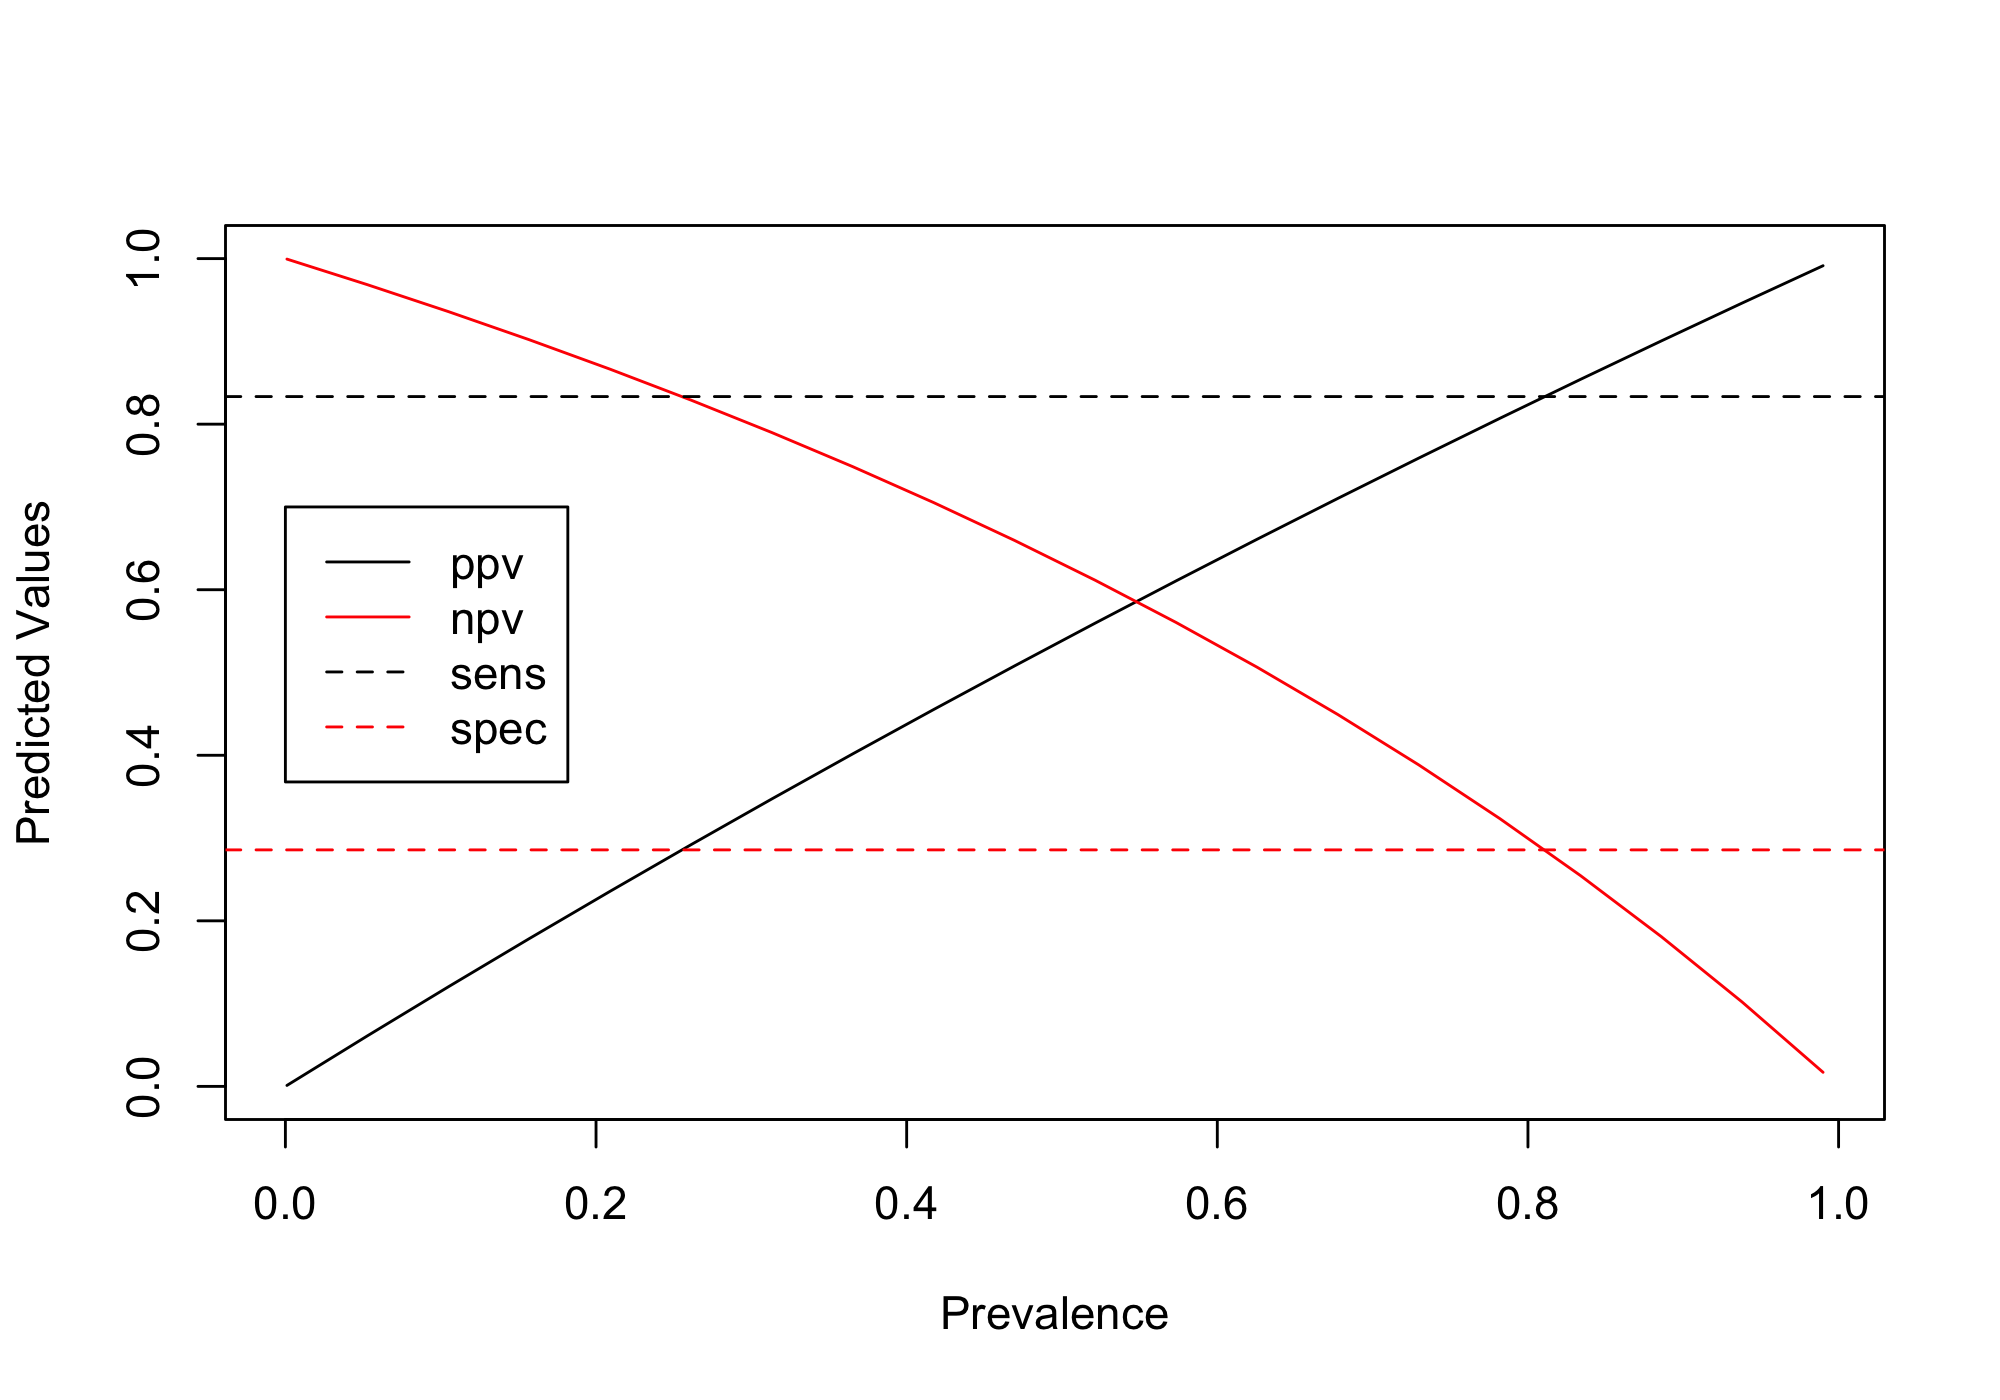
\includegraphics[scale=0.19]{img/plot}
			\captionof{figure}{Plots of the probability values for sample size}
			\label{fig:prevalence}
		\end{center}
	\end{figure}
	
	Continuing with the example in \citet{archit2020} of pool testing, and let the probability that a person living in Mexico has COVID-19 is 0.007 (as calculated before) to 0.012. If it is pooled $ x $ samples and probability that a person has the disease is $p$, then the probability that at least 1 person will have covid is given by:
	
		\begin{equation}
		P  = 1 - (1-p)^{x}.
	\end{equation}

	If it is an interest to know the probability that at least 1 person has COVID-19, from a pool of x samples tested positive, to be more than 99\% or might be less; Bayes' Theorem can also be applied. This result can be shown in Figure \ref{fig:sample_plot}, which can be used to choose the number of samples for pool testing.

		\begin{figure}
		\begin{center}
			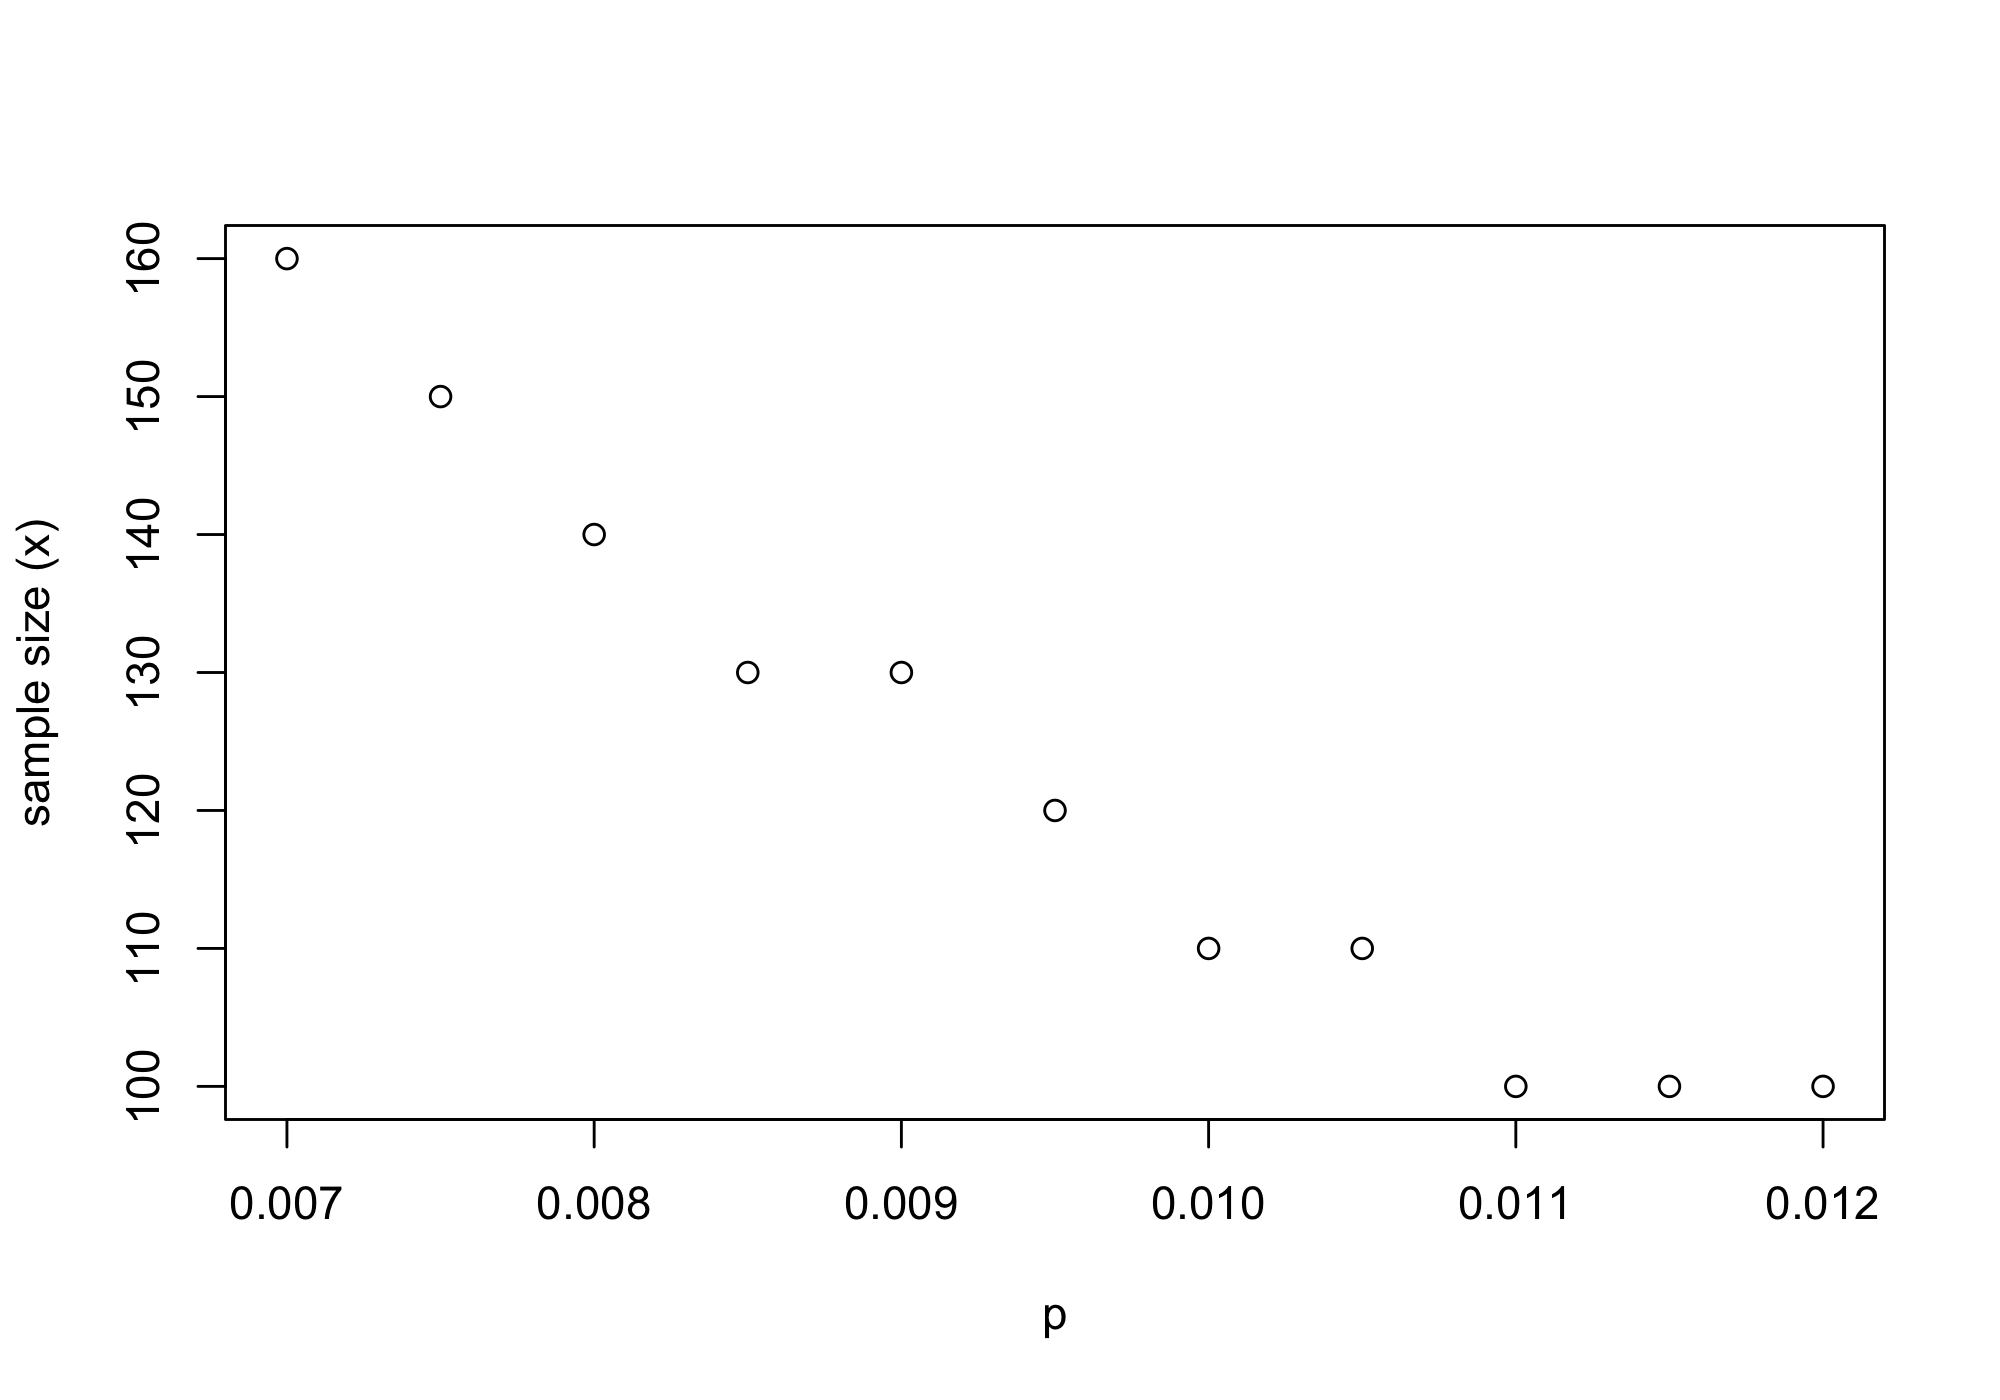
\includegraphics[scale=0.19]{img/sample_plot}
			\captionof{figure}{Plots of the probability values for sample size}
			\label{fig:sample_plot}
		\end{center}
	\end{figure}
		
\clearpage

	\bibliography{assignment8}
	\bibliographystyle{plainnat}
	
\end{document}